\documentclass[../FGP.tex]{subfiles}
\begin{document}
\setmarginpargeometry
\part*{Research \& Inspiration}
\addcontentsline{toc}{part}{Research \& Inspiration}
\section{Research Notes}
\subsection{Reading List}
This section is modestly misleading, this is not a bibliography of all sources these notes reference. Instead this is more like a to-do list for things I have not read yet, or have read in little bits but not cited in the text, or may need to remember on background but might never actually directly cite in text. It is annotated so I may remember \emph{why} I need to read these in more detail later. 
\subsubsection{Aristotle}\label{biblio:aristotle}
\begin{annotated-bibliography}
  \item Frank N.~Egerton, \textit{Changing Concepts of the Balance of Nature}, 48 \textsc{Q.~Rev.~Biology} 322, 327-29 (1973) (unusually among ancient philosophers, Aristotle doesn't have a vision of nature as self-regulating. Rather, the telos unique to each animal governs the behavior other philosophers attributed to nature's ability to self-balance).
  \item Armando Aranda-Anzaldo, \textit{Aristotle and the search of a rational framework for biology}, 3 \textsc{Organisms: J.~Biological~Sci.s} 54 (2019) (claiming Aristotle does have a notion of equilibrium at the organism level) 
  \item Giora Hon \& Bernard R. Goldstein, \textit{What Keeps the Earth in Its Place? The Concept of Stability in Plato and Aristotle}, 50 \textsc{Centaurus} 305 (2008) (exploring Aristotle's concept of ``natural place'' and contrasting it to modern notions of equilibrium in physics which rely on symmetry)
  \item James M.~Rhodes, \textit{Right by Nature}, 53 \textsc{J.~Pol.} 318 (1991) (implicitly arguing that the right shape of a polity is constrained by the right shape of human life, because it must ``habituate[] citizens to the virtues'').
  \item Dylan B.~van der Schyff, \textit{The Ethical Experience of Nature: Aristotle and the Roots of Ecological Phenomenology}, 4 \textsc{Phenomenology \& Prac.} 97 (2010) (arguing Aristotle's understanding of a thing's nature has many traits of the phenomenological, not actually sure how useful this article is).
\end{annotated-bibliography}

\subsubsection{Thomas Aquinas}\label{biblio:thomas}
See also \textsc{Ptolemy of Lucca} in the Mirror for Princes section,\footnote{\textit{infra} \ref{biblio:mirrorforprinces}.} which is chiefly of interest for portions that may or may not have been written by Thomas Aquinas.
\begin{annotated-bibliography}
  \item Joaquin F.~Garcia, \textit{Thomist Natural Law}, 8 \textsc{Cath.~Law.} 31 (1962) (broad review of Thomas Aquinas' understanding of the relation between reason and positive law)
  \item Michael W. Tkacz, \textit{Thomistic Reflections on Teleology and Contemporary Biological Research} 94 \textsc{New Blackfriars} 654 (2013)] (arguing that -- in practice -- modern biology relies heavily on teleological explanations for how species are adapted to particular niches)
\end{annotated-bibliography}
\subsubsection{Mirrors for Princes}\label{biblio:mirrorforprinces}
\begin{annotated-bibliography}
  \item \textsc{Ptolemy of Lucca with portions attributed to Thomas Aquinas}, \textsc{On the Government of Rulers: De Regimine Principum} (James M.~Blythe trans., Univ.~Penn.~Press 1997)(c.~1265) (sections up to \S2.4, maybe by Aquinas, applying Aristotle's \textit{Politics} to describe obligations of kings; later portions of interest for an Aristotelian-motivated perspective skeptical of monarchy)
  \item \textsc{Desiderius Erasmus}, \textsc{The Education of a Christian Prince with the Panegyric for Archduke Philip of Austria} (Lisa Jardine trans., Cambridge Univ.~Press 1997) (1532) 
  \item \textsc{Niccolò Machiavelli, The Prince} (Harvey C.~Mansfield, trans., Univ.~Chi.~Press 2d ed. 1998) (1532) (advice specifically for \emph{new} Princes who cannot rely on legitimacy from a regal line that has long ruled in their territory).
  \item Lester K. Born, \emph{Erasmus on Political Ethics} 43 Pol. Sci. Q. 520 (1928) (Listing many more examples of mirror-for-princes lit)
  \item \textsc{Aysha Pollnitz}, \textsc{Princely Education in Modern Britain} (2015) (chapter three of particular interest for tracing the influence of \textsc{Erasmus} \textit{supra}, on Henry VIII's claims to supremacy over papal authority).
\end{annotated-bibliography}

\subsubsection{Machiavellianism}
\begin{annotated-bibliography}
\item Stuart Hampshire, \textit{Morality and Pessimism}, \textit{in} \textsc{Public \& Private Morality} 1 (Stuart Hampshire ed., 1978)(Argues for a particularist view of morality where our moral commitments are made in comparison with asking what kind of person we want to be and by reflecting and refining our natural intuitions about the moral valence of an act, criticises the influence of utilitarianism on public policy as legitimating monstrosities and for vulgar utilitarianism not really resembling an ethical system in that it's devoid of ethical primitives. Also takes as a central argument that human ability to compute the utilitarian consequences of an action has stalled and therefore utilitarianism cannot be a progessive philsophy as it once was. I don't know if there's a ton of useful info I can grab from this, but one interesting thought is the way that being in-the-know or not about Hylia's role may give Zelda and her retinue a completely different set of ethical primitives than the average Hylian, which may or may not be worth exploring).

\item Stuart Hampshire, \textit{Public and Private Morality}, \textit{in Id.} 23 (attempts to make more precise critiques offered in \textit{Morality and Pessimism}, \textit{supra}. Previous article didn't feel terribly applicable so I've skipped this at least for now). 

\item Bernard Williams, \textit{Politics and Moral Character}, \textit{in Id.} 55 (attempts to ask and answer what kind of person we want making political decisions, with a very rewarding defence of the inevitability of ethical dilemmas in political action at 61--64)

\item Thomas Nagel, \textit{Ruthlessness in Public Life}, \textit{in Id.} 75 

\item T.~M.~Scanlon, \textit{Rights, Goals, and Fairness}, \textit{in Id.}, 93

\item Ronald Dworkin, \textit{Liberalism}, \textit{in Id.}, 113
\end{annotated-bibliography}

\subsubsection{Religious Belief of Commoners}
\begin{annotated-bibliography}
\item \textsc{Carlo Ginzburg, The Cheese and the Worms: The Cosmos of a Sixteenth Century Miller} (John Tedeschi \& Anne Tedeschi trans., John Hopkins Univ. Press 1980) (1976) (A possibly useful comparison for theological expression in another case where -- if you didn't speak Latin -- much of the world's cosmology was inaccessible)\begin{description}
\item[20:]\hspace{.25em} useful notes about an urban-rural divide in religion
\item[28--36:]\hspace{.25em} notes about what books were available to Scandella, how he came to have them, and notable features of how Scandella's prior outlook shapred his interpretation of the books
\item[50:]\hspace{.25em} Of interest for multi-directional efforts of censorship on the part of the church -- i.e., both high and low culture, which intermix quickly.
\item[59:]\hspace{.25em} has a high-level contrast of things which are understood through written culture vs oral culture which might bear most directly on what you're trying to do
\item[60--61:]\hspace{.25em} Some juicy bits concerning the way printing made philosophical knowledge accessible in a patchwork kind of way, this may integrate very well with the Book of Mudora as a trope in LttP (i.e., a semi-publically available chrestomathy which gives patchwork access to lore).
\end{description}
\end{annotated-bibliography}

\subsubsection{Witchcraft}
\begin{annotated-bibliography}
\item Peter Laslett, \textit{Sir Robert Filmer: The Man versus the Whig Myth}, 5 \textsc{Wm.~\& Mary Q.} 523 (1948) (complicating Filmer's conservatism by comparing it against his relative progressivism on questions such as ``Witchcraft: Is it a Thing?'')
\item \textsc{Robert Filmer}, \textsc{An Advertisement to the Jury-Men of England Touching Witches Together with a Difference between an English and Hebrew Witch} (The Rota 1975)(1643)(disputing that it is easy to identify who is a witch using the definition then in operation)
\item \textsc{William Perkins}, \textsc{A
Discourse
of the Damned
Art of Witchcraft;
so farre forth
as it is Revealed in the Scriptures, and
Manifest by True Experience} (1610), \textit{available at} \url{https://quod.lib.umich.edu/e/eebo/A09402.0001.001?rgn=main;view=fulltext} (arguing for a consistent definition of witchcraft as compact with devil since antiquity).
\end{annotated-bibliography}

\subsubsection{Cats}
\begin{annotated-bibliography}
\item Daria L. Clark \& Robert A. Clark, Neutral point testing of color vision in the domestic cat, 153 \textsc{Experimental Eye Rsch.} 23 (2016) (``These results provide strong evidence that cats are dichromatic with a neutral point near 505 nm. This neutral point is nearly identical to the neutral point of the human deuteuranope, making feline vision a more accurate a model for red-green colorblind individuals than normal trichromats.'')
\end{annotated-bibliography}
 
 \subsubsection{Language}
 \begin{annotated-bibliography}
 \item \textsc{Joseph Bosworth, An Anglo-Saxon Dictionary} (Thomas Northcote Toller, Christ Sean, and Ondřej Tichy, eds. 2014) (1898)
 \end{annotated-bibliography}
\subsection{Commonplace}

\subsubsection{Magic}
Useful for figuring out the fortune telling scenes at a high level of ``what kind of fortune can be told?'': \begin{quote}
``There is a natural course through life that every subject \emph{would} follow if nothing took place to change it, and no effort was made to improve. In other words, we believe there is a general outline of the course and limitations of the life of the subject. This general course is what the subject would \emph{naturally} do through life, because of the combination of type qualities which he possesses.''\footnote{\textsc{William G.~Benham, The Laws of Scientific Hand Reading} 374 (Health Research Books, 1993) (1901)}
\end{quote}Meanwhile this is useful for fears about an early demise on one adventure or another:
\begin{quote}
While no sign is seen on the Life line, a deep cut or cross, a dot or a star, may be discerned on the Head line corresponding to the age at which the Life line ends, and this will be the sign of the demise.\footnote{\textit{Id.} at 499.}
\end{quote}
\subsubsection{Political Authority}
This might be useful for your comment on destinies/natures: ``Men also adopt different methods in proceeding towards their proposed end, as the diversity of men’s pursuits and actions clearly indicates. Consequently man needs some directive principle to guide him towards his end.''\footnote{\label{note:aquinas}\textsc{Thomas Aquinas, On Kingship: To the King of Cyprus}, (Gerald B. Phelan, trans., I. Th. Eschman \& Joseph Kenny, eds.), \P1 \textit{available at} \url{https://isidore.co/aquinas/DeRegno.htm} (herein \textsc{On Kingship})} (Of interest here because it seems to be saying that there is a single end for men, but broadly differentiated notions of how to pursue it, which mirrors and tracks some of the thinking you've been developing about what the goddesses have in mind for most destinies, and of interest to me because this is a nuance I don't recall showing up in the Politics.).

``I say, then, that in hereditary states accustomed to the bloodline of their prince the difficulties in maintaining them are much less than in new states because it is enough not to depart from the order of his ancestors, and then to temporize in the face of accidents. In this way, if a prince is of ordinary industry, he will always maintain himself in his state unless there is an extraordinary and excessive force which deprives him of it; and should he be deprived of it, if any mishap whatever befalls the occupier, he reacquires it.''\footnote{\textsc{Niccolò Machiavelli, The Prince}, 6--7 (Harvey C.~Mansfield, trans., 2d ed., 1998) (Translator's footnotes omitted.)}

``Thus an hereditary system, which by definition presupposed a settled situation where the loyalties and the expectations of the subjects remained fairly constant, did not call for any special skill or knowledge and hence presnted no real challenge to political science.''\footnote{\textsc{Sheldon Wolin, Politics and Vision: Continuity and Innovation in Western Political Thought}, 179 (expanded ed., 2004)}

``The Lord, therefore, threatens such rulers, saying by the mouth of Ezekiel: `Woe to the shepherds that feed themselves (seeking, that is, their own interest): should not the flocks be fed by the shepherd?' Shepherds indeed should seek the good of their flocks, and every ruler, the good of the multitude subject to him.''\footnote{\textsc{On Kingship}, \textit{supra} note \ref{note:aquinas} (quoting \textit{Ezekiel}, 34:2), \textit{but see} Thrasymachus' objection in \textsc{Plato, Republic}, 19 (G.M.A.~Grube, trans., C.D.C.~Reeve rev., 1992) (Stephanus 343a--b, ``You think that shepherds and cowherds seek the good of their sheep and cattle, and fatten them and take care of them, looking to something other than their master's good and their own,'' but actually shepherds care for the sheep only to fatten themselves.) -- an objection which Socrates attempts to rebut by saying that insofar as a person seeks their good rather than that of the sheep, they are not being a shepherd, \textit{id.,} at 21 (345c--d), but I do not think this rebuttal is successful, and \textit{cf.} against \textsc{On Kingship}, \P 103 (``Thus a ship is said to be governed when, through the skill of the pilot, it is brought unharmed and by a direct route to harbour. Consequently, if a thing be directed to an end outside itself (as a ship to the harbour), it is the governor’s duty, not only to preserve the thing unharmed, but further to guide it towards this end.''), which makes it unclear why the the flock cannot have the dinner table as an external end, except maybe that sheep are animate and their own ends are the more important consideration. Maybe implicit in this metaphor is the idea that the ends of the flock must closely follow the ends of the sheep, or the supposition that an (internal) end cannot destroy the thing which has it as an end. It is a tragedy the Lyceum never found out about praying mantises. Anyway, I don't know that knocking down the shepherd-flock analogy makes much difference for the original claims about the nature of kingship, but the analogy itself seems very obviously wrong and annoys me no end.}

\begin{verse}
\textsc{Exton:} 
``Have I no friend?" quoth he. He spake it twice\\
And urged it twice together, did he not?

\textsc{Servingman:}  He did.

\textsc{Exton:} And speaking it, he wishtly looked on me,\\
As who should say ``I would thou wert the man\\
That would divorce this terror from my heart''—\\
Meaning the king at Pomfret. Come, let’s go.\\
I am the King’s friend and will rid his foe.\footnote{\textsc{William Shakespeare, Richard II} act 5, sc. 4, l. 5--12.}
\end{verse}

\section{Shippy}
The entirety of \textit{The Ballad of Pertinent Information (Turn It On))}\footnote{\textsc{The Paranoid Style}, \textit{The Ballad of Pertinent Information (Turn It On))}, \textit{on} \textsc{The Interrogator} (Bar/None 2024), \textit{available at} \url{https://theparanoidstyle.bandcamp.com/track/the-ballad-of-pertinent-information-turn-it-on}.} is just tone-perfect for Irene's feelings: disenchanted and ebullient, cynical and adoring, skeptical of the relationship but diving head-first anyway, but of all of it I think \begin{verse}
Turn it on (I must be either Pratt or Whitney)\\
Turn it on (Some kinds of folks would give you a kidney)\\
Turn it on (My mind wanders and my ears ring)\\
Turn it on (I would give you everything)
\end{verse} is maybe my favorite verse in a long time, and easily the one best suited to this fic. 

\begin{figure}
  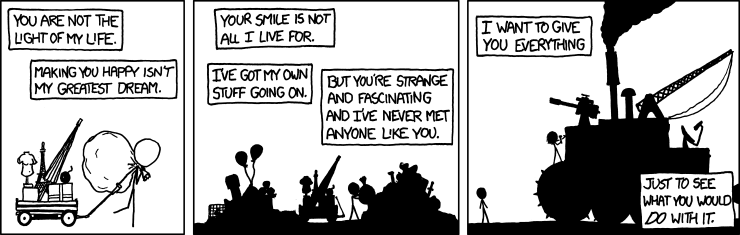
\includegraphics[width=\textwidth]{../lib/everything}
  \caption{Randall Munroe, \textit{Everything}, \textsc{xkcd} (Oct. 24, 2011), \url{https://xkcd.com/968/} (the comic is given the hover-text: ``I wanna hold your hand so I don't fall out of your gyrocopter.'')}
\end{figure}


\end{document}

